\documentclass{article} % For LaTeX2e
\usepackage{nips13submit_e,times,graphicx}
\usepackage{hyperref}
\usepackage{url}
%\documentstyle[nips13submit_09,times,art10]{article} % For LaTeX 2.09

\nipsfinalcopy
\title{Learning the Language of the Genome using RNNs}


\author{
Jesse M. Zhang \\
Department of Electrical Engineering \\
Stanford University \\
Stanford, CA 94305 \\
\texttt{jessez@stanford.edu} \\
\And
Govinda M. Kamath \\
Department of Electrical Engineering\\
Stanford University\\
Stanford, CA 94305 \\
\texttt{gkamath@stanford.edu} \\
}

% The \author macro works with any number of authors. There are two commands
% used to separate the names and addresses of multiple authors: \And and \AND.
%
% Using \And between authors leaves it to \LaTeX{} to determine where to break
% the lines. Using \AND forces a linebreak at that point. So, if \LaTeX{}
% puts 3 of 4 authors names on the first line, and the last on the second
% line, try using \AND instead of \And before the third author name.

\newcommand{\fix}{\marginpar{FIX}}
\newcommand{\new}{\marginpar{NEW}}

%\nipsfinalcopy % Uncomment for camera-ready version

\begin{document}


\maketitle

\begin{abstract}
We explore how deep recurrent neural network (RNN) architectures can be used to capture the structure within a genetic sequence. We first confirm that a character-level RNN can capture the non-random parts of DNA by comparing the perplexity obtained after training on a real genome to that obtained after training on a random sequence of nucleotides. We then train a bidirectional character-level RNN to predict whether a given genomic sequence will interact with a variety of transcription factors, DNase I hypersensitive sites, and histone marks. Because multiple biological objects can interact with a given sequence, we cast this latter problem as a multitask learning problem. We empirically show how a deep network can outperform a baseline model a significant majority of $919$ binary labeling tasks. 
\end{abstract}

\section{Introduction}
In recent years, deep recurrent neural networks (RNNs) have allowed researchers to tackle a variety of machine learning problems in the domain of natural language processing. Most of these applications investigate problems such as translation, named entity recognition, and sentiment analysis. Less work has been done with RNNs on what is perhaps the most natural language: the genome, a sequence of four letters (A, C, G, T). The purpose of this project is to explore how an RNN architecture can be used to learn sequential patterns in genomic sequences.

To confirm that an RNN can model the structure within a genomic sequence, we first train a simple character-level RNN to predict one of the four possible characters given the previous string of characters. If the ability of an RNN to predict the next character for a real genome is the same as for a random genome, then we will have to more carefully tweak our model until we can identify some signal. We will also use this simpler task to help choose a proper model architecture.

Once we have empirical evidence that an RNN can capture the non-random structure within a genome, we explore a sequence classification problem. Epigenetics is the study of how the genome is regulated by external factors. Biological experiments have shown that subsequences of the human genome are often regulated by both nearby and very distant sequences Specifically, biologists have been able to identify whether a particular genomic feature will be observed for a particular sequence. Examples of these features include
\begin{enumerate}
	\item Transcription factors: proteins that bind to a particular sequence
	\item DNase I hypersensitive sites: a sequence that is sensitive to cleavage by the DNase I enzyme
	\item Histone marks: chemical modifications to histone proteins, biomolecules  which regulate certain sequences.
\end{enumerate}

These results are available via the ENCODE \cite{encode2012integrated} and Roadmap Epigenomics \cite{kundaje2015integrative} data releases. For each of many features, we will assess an RNN's ability to predict whether a given feature will be present based solely on the sequence.

\section{Related work}

Several deep genomic models have emerged in the past year, and the ones discussed below attempt to predict whether a certain genomic feature will be observed at a particular sequence.

Two tools were published in August 2015. DeepSEA \cite{zhou2015predicting} performs prediction based solely on a fixed-length genomic sequence. The authors use a deep convolutional neural network (CNN) over an input sequence, alternating between convolutional and pooling layers to extract sequence features. They use a sigmoid output layer to compute the probability of seeing a particular genomic feature. DeepBind \cite{alipanahi2015predicting} also uses a deep CNN with 4 stages of convolution, rectification, pooling, and some nonlinearity. Unlike for DeepSEA, DeepBind accommodates varying-length inputs and also incorporates extra information in addition to just the input sequence. This extra information comes from known facts about a particular sequence gathered from other experiments. Basset \cite{kelley2015basset} was published a few months later in October 2015. This tool likewise uses a deep CNN architecture to learn the functional activity of genomics sequences.

DanQ \cite{quang2015danq}, published in December 2015, incorporates a bidirectional long-short-term-memory (LSTM) RNN on top of the outputs of a max pooling layer after convolution on the input sequence.

Each of these tools feeds a one-hot encoding of an input sequence into a convolution layer. In other words, the networks operate on a $4\times L$ matrix obtained from a length-$L$ sequence. 

\section{Approach}

All RNN models in this project were built using Google's \texttt{TensorFlow} Python package. For the character-level genome modeling task, we tested a variety of RNN-based neural network architectures including gated recurrent units (GRUs) and long-short-term-memory RNNs (LSTMs). We experimented with a variety of hyperparameters on multiple genomes in order to assess the robustness of a given model. We will measure the ability of a model to fit a given dataset using the average perplexity across all character prediction tasks:

$$
	PP(\mathbf{y},\mathbf{\hat{y}}) = \exp \left\{-\frac{1}{n-1} \sum_{t=1}^{n-1} \sum_{i=1}^{|V|} y_i^{(t)} \log \hat{y}_i^{(t)}\right\}
$$

where $n$ is the number of training samples (roughly the length of our genome), $|V|$ is the size of our vocabulary, $\hat{y}^{(t)}_i$ is the predicted probability of the predicted word at time $t$ being word $i$, and $\mathbf{y}^{(t)}$ is a one-hot vector describing the actual word at time $t$.

From the above experiment, we selected a cell type to use for the multitask learning model. We used a bidirectional GRU for character-level processing. Each character in the input sequence is mapped to some low-dimensional embedding. Intuitively, a genetic sequences can be regulated by both flanking sequences, and therefore bidirectionality is a crucial part of the architecture. The outputs of the forward and backward RNNs are fed through a softmax layer. For each of $K$ tasks, a prediction of 0 or 1 is made, indicating whether or not a particular feature should be observed for the input sequence. For all tasks, all weights are shared before the final softmax. Each task has its own weight and bias matrices at the softmax layer. The overall architecture is summarized in Figure 1. The overall loss is the geometric mean of the perplexity across all $K$ tasks. 

\begin{figure*}[!htb]
	\centering
	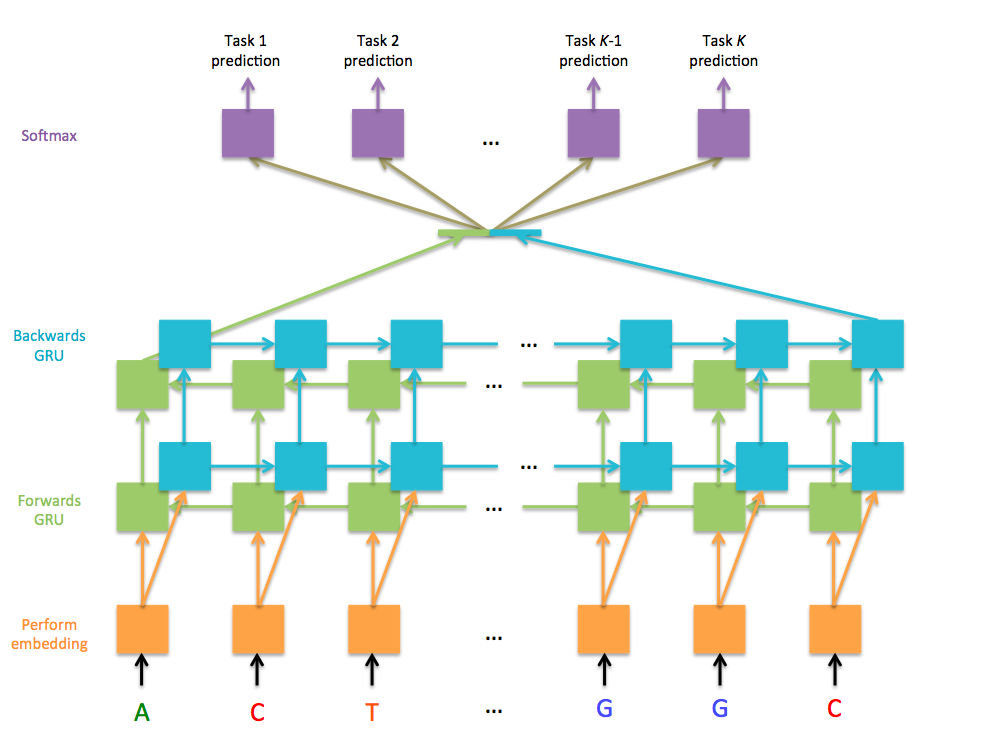
\includegraphics[scale=0.4]{Figure1}
	\caption{The network architecture used to perform multitask prediction for a given input genomic sequence. Each character in the input sequence is mapped to a low-dimensional embedding, which is fed into a bi-directional recurrent neural network consisting of gated recurrent units. The outputs of the last GRU in the forwards and backwards RNNs are concatenated before being fed to one of $K$ prediction tasks. A final prediction of 1 or 0 is made for each task.}
\end{figure*}

\section{Experiment}

Experimentation was performed by first gathering datasets of synthetic genomes, real genomes, and sequence-label training examples. Due to the size of the training set for the multitask prediction problem, we used a simpler problem (genome character-level prediction) to choose certain hyperparameters. Our evaluation metric was based on the perplexity cost function above for non-classification tasks and an F1 score for classification tasks. For the multitask prediction problem, we implemented a baseline that involved both feature extraction and logistic regression.

\subsection{Dataset}

For the character-level genome prediction task, four genomes were prepared:
\begin{enumerate}
	\item A length-30,000 repeating genome where the repeated unit is \texttt{AGCTTGAGGC}
	\item A length-30,000 random genome
	\item The length-4,639,675 genome for \textit{E. coli}
	\item The length-23,264,338 genome for \textit{P. falsifarm}
\end{enumerate}


For the multitask prediction task, we used a random subset of the dataset used in the DanQ \cite{quang2015danq} and DeepSEA \cite{zhou2015predicting} papers. The dataset was collected from experiments reported in the ENCODE \cite{encode2012integrated} and Roadmap Epigenomics \cite{kundaje2015integrative} data releases. We chose 80,000 sequence-label pairs for the training set, 8000 pairs for the testing set, and 2000 for the validation set. Each sequence has a length of exactly 1000. All sequences are length-200 subsequences of the human genome with 400 bp flanking regions. The length-200 portion is nonoverlapping across different sequences. The set of labels describes 919 binary prediction tasks, and each indicates whether part of a particular sequence was observed as accessible for a particular ChIP-seq or DNase-seq experiment (i.e. if a ChIP-seq or DNase-seq peak for a particular experiment overlaps with the 200-bp region by at least half of the length of the peak). Both of these types of experiments evaluate the locations where one of the three features (see introduction) can bind. The dataset is noisy, and about 10\% of the tasks' labels were all 0. In general, tasks are strongly skewed towards negative examples. For 421 of the 919 tasks, less than 1\% of the training examples were labeled 1.

Due to computational limitations, training an RNN on all 1000 characters in each example was difficult. The RNNs discussed below were instead trained on the middle 100 characters of each sequence. For a fair comparison, the baseline model was trained on the same set of truncated sequences. 

\subsection{Character-Level Genome Prediction Results}

For this task, our baselines were the artificial genomes (first two genomes in the list). Any model that does not perform as expected on these two genomes will not be used on other genomes. We wanted to perform better than the random genome, and the repeating genome serves as an empirical lower bound. For these genomes, we used an LSTM architecture, a dropout keep rate of 1, a batch size of 50, a sequence length of 50, a learning rate of 0.002, and 10 epochs. The achieved perplexity of the random genome was 4.003, just as expected. This is the case when the model always assigns equal probability to each of the 4 possible character A, C, G, T. The achieved perplexity of repeating genome is 1.002, which was also just as expected. Since the sequence repeats without noise, we expect the model to be able to put all the probability mass on a single character.

For the \textit{E. coli} and \textit{P. falsifarm} genomes, we used a dropout keep rate of 1, a batch size of 50, and 1 epoch. We tested the GRU, LSTM, and RNN architectures, learning rates of 0.0001 and 0.0008, sequence lengths of 50, 100, 500, and 1000, and 2 and 3 layers. The number of epochs was limited to 1 in order to quickly test every combination of the above hyperparameters. For both genomes, all combinations of hyperparameters performed about the same, reaching a perplexity of 3.679 for \textit{E. coli} and a perplexity of 2.938 for malaria. All training errors were continuing to decrease after 1 epoch, however, indicating that increasing the epochs will allow for even smaller perplexities (Figures 1 and 2).

The learning rate of 0.0001 performed worse than the learning rate of 0.0008, but this is likely because the former is slower at updating. Both 2 and 3 layers worked about the same. Surprisingly, 50 or 100-length sequences perform better than 500 or 1000-length sequences despite the fact that genomes often involve long-range interactions. Finally, both RNNs and GRUs appear to outperform LSTMs.

While the perplexity being less than random is reassuring, the results obtained here are not useful by themselves. Genomes are known to have repeat structures in certain regions. This and the fact that that there existed an unequal distribution of the four nucleotides can produce a lower perplexity. Nevertheless, these experiments showed that a 2 layer network using GRUs may be appropriate for modeling a genomic sequence. These will be used for training a model to handle the primary problem in this project: multitask prediction.

\subsection{Multitask Prediction Baseline and Evaluation Metric}

Just as in \cite{quang2015danq}, a baseline was drawn by first mapping each sequence in the training set to a feature vector and then running the vector-label pairs through a simple logistic regression model. The first feature mapping used involving mapping each of the 4 nucleotides to an integer 0, 1, 2, or 3. As expected, this feature mapping performed quite poorly as the mapping fails to capture how adjacent characters interact.

Instead, we used a feature mapping inspired by the authors of \cite{quang2015danq}. We used a $k$-mer bag of words method where each length $k$ subsequence of an input sequence was counted. We used $k = 1, 2, 3, 4, 5$, resulting in $4^1 + 4^2+4^3+4^4+4^5 = 1364$ features. For example, the sequence \texttt{ACTGG} would produce a length-1364 feature vector where the entries corresponding to the $k$-mers \texttt{A}, \texttt{C}, \texttt{T}, \texttt{AC}, \texttt{CT}, \texttt{TG}, \texttt{GG}, \texttt{ACT}, \texttt{CTG}, \texttt{TGG}, \texttt{ACTG}, \texttt{CTGG}, and \texttt{ACTGG} would each equal 1, and the entry corresponding to \texttt{G} would equal 2. All other entries equal 0.

Logistic regression was performed using the Python module \texttt{scikit-learn}. Default parameters were used except for the regularization constant of the $\ell_2$ regularization term, which was set to $10^{-6}$. A separate logistic regression model was trained for each of the 919 tasks on all 80,000 training examples (with length-100 sequences). The performance of a model was evaluated based on the its prediction accuracy on the 8000 training examples. Note that a validation set was not used here; each logistic regression model was simply trained until the default tolerance of 0.0001 was reached. Because all examples are severely skewed towards the 0 class (i.e. for all tasks, there are significantly more examples without the feature than with the feature), the raw error rate is not a good indicator of prediction accuracy. We instead looked at the F1 score, defined as:
$$ F_1 = 2 \cdot \frac{\mbox{precision} \cdot \mbox{recall} }{\mbox{precision} + \mbox{recall}} $$

where precision is the proportion of correct positive predictions, and recall is the proportion of positive examples that received a positive prediction. 

To account for the fact that less than 1\% of the training examples were labeled 1, we looked only at tasks where at least 1\% of the training examples were labeled 1 (498 of the 919 tasks).

\subsection{Multitask Prediction Results}

The final model used a learning rate of 0.001 for an Adam Optimizer, 2 layers, an embedding size of 2 (as there were only 4 unique characters), hidden layer sizes of 128, a dropout keep probability of 0.95, and batch size of 20. The RNN was bidirectional and used GRU units with tanh activation function. The RNN processed all 100 characters of each input sequence. The model was trained for 61 epochs on the 80,000 training examples, running for approximately 3 days using an NVIDIA GRID K520 GPU on an Amazon Web Services Elastic Compute Cloud instance.

Figure 2 shows how the loss function (average perplexity across all examples and tasks) changes for both the validation and test sets as the number of epochs increases. We see that while the training loss continues to decrease, the validation loss has plateaued around a perplexity of 1.087.

\begin{figure*}[!htb]
	\centering
	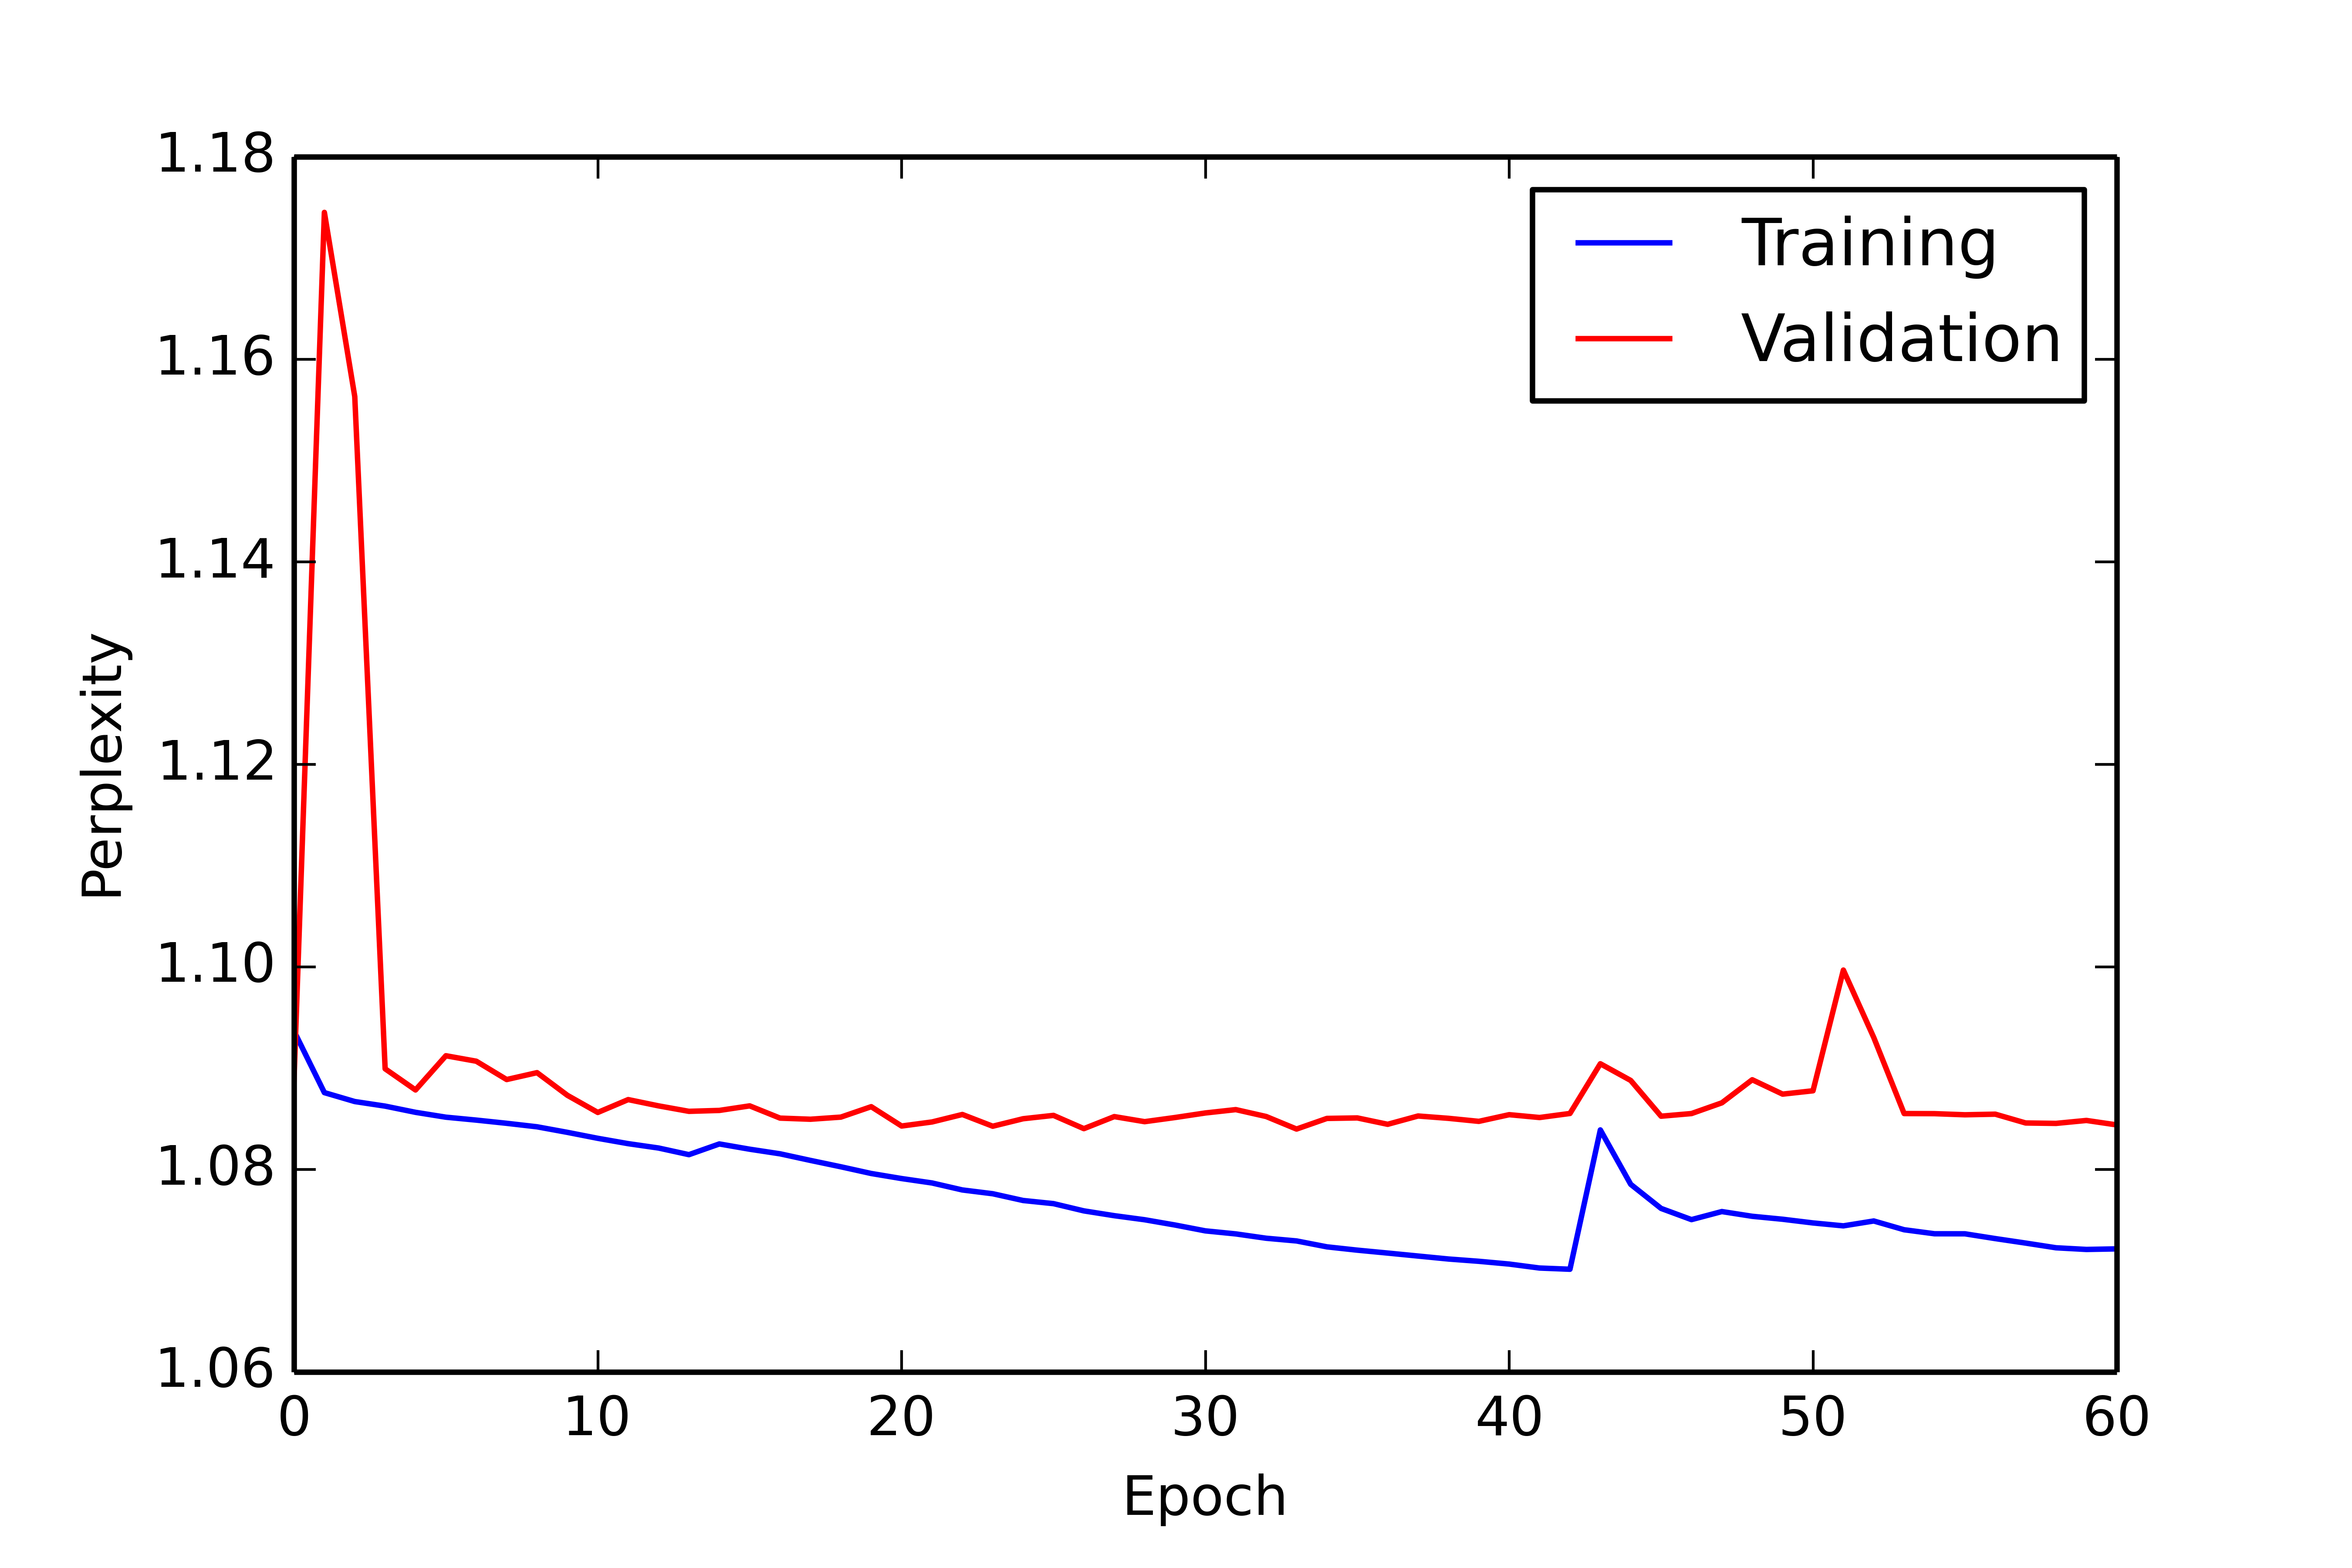
\includegraphics[scale=0.6]{loss_100}
	\caption{The training and validation losses as functions of number of training epochs for the bidirectional RNN model. Training was done with 80,000 length-100 sequences across 919 binary labeling tasks.}
\end{figure*}

The weights from all epochs were tested on the test set. Figure 3 shows the F1 scores for logistic regression (blue) and the RNN with weights corresponding to the lowest validation perplexity (green). We also show the max F1 score achieved across all weights from all training epochs.

\begin{figure*}[!htb]
	\centering
	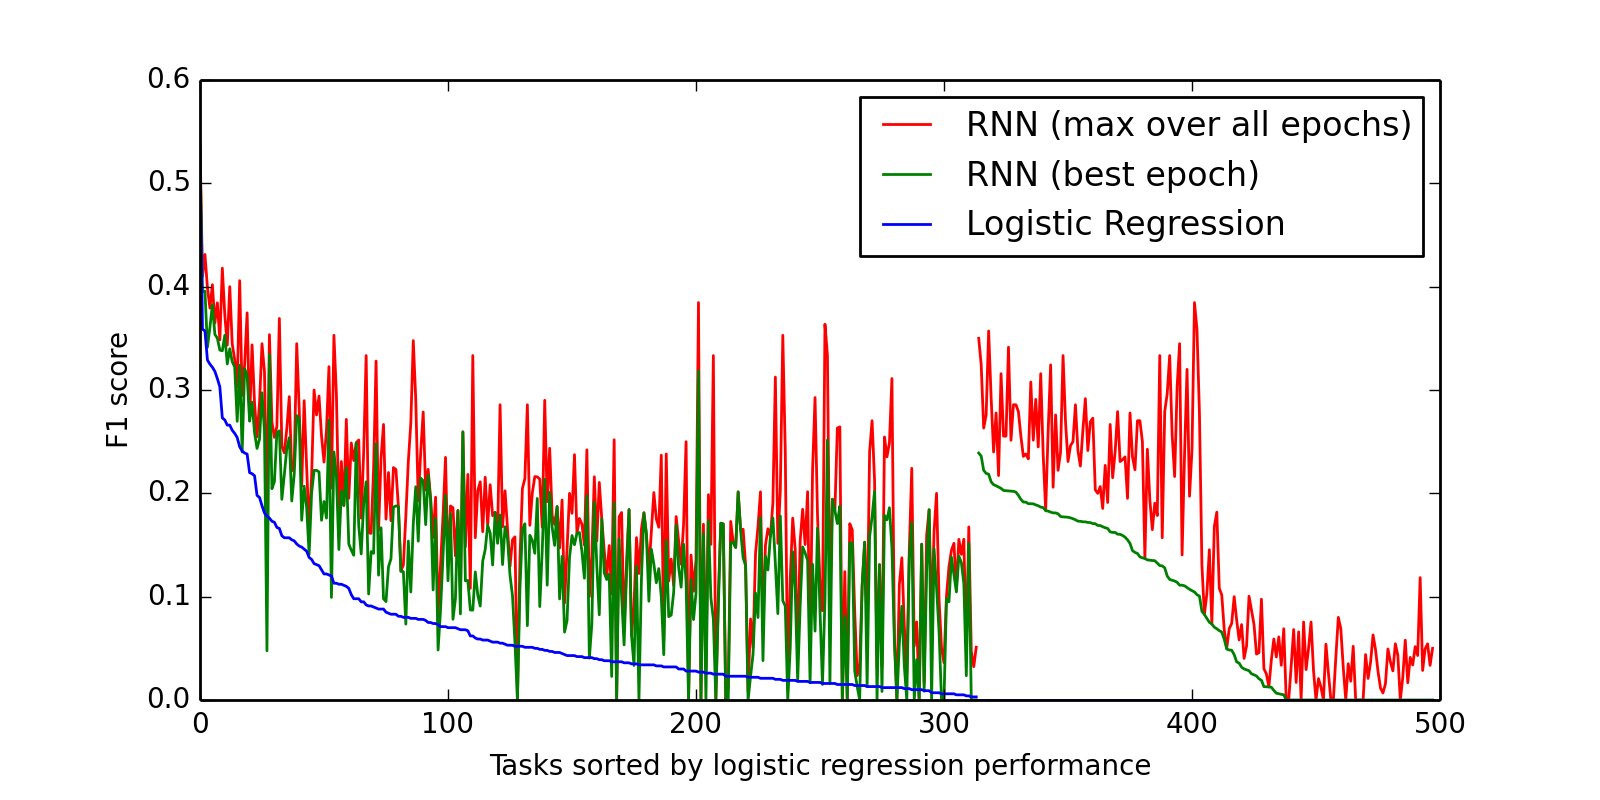
\includegraphics[scale=0.6]{F1_scores_498}
	\caption{F1 scores for the logistic regression and RNN models for the 498 tasks with at least 800 positive training examples (out of 80000 total examples). The RNN epoch corresponding to the lowest validation error was epoch 33. Tasks where logistic regression achieved an F1 score of 0 were sorted instead by the F1 scores of the RNN with weights from epoch 33.}
\end{figure*}

The RNN's optimal weights were achieved at epoch 33. For 498 tasks where at least 1\% of the training examples were labeled 1, the RNN with epoch 33 weights achieved a higher F1 score for 408 or 81.9\% of the tasks. On average, the RNN achieved scores that were greater by 0.091. Taking the max F1 score for each task over all epochs, the RNN beats logistic regression in 471 or 94.6\% of the tasks, achieving F1 scores that were greater by 0.131 on average. When enough positive training examples are present, the RNN outperforms the logistic regression baseline for the classification problem.

For the 421 tasks with less than than 800 positive examples in the training set, the optimal weights won on 43.2\% of the tasks, and the maximum F1 score over all epochs won on 65.6\% of the tasks. With so few positive training examples for these tasks, we expect the RNN to suffer a significant decrease in performance because RNNs are notoriously dependent on large amounts of training examples. Despite this, the correlation between tasks likely allowed the RNN to leverage examples from other tasks to learn more about a given task, resulting in comparable performance from the RNN.

Additionally, taking the max F1 scores over all epochs results in significant performance gains over using just the weights at any one epoch. This suggests the model sacrifices accuracy for some tasks in order to gain accuracy for other tasks. With 919 tasks, this may not be too surprising. More nodes at the hidden layer could alleviate this, but we would need more time for training.

\section{Conclusion}
In this project, we used RNNs to perform character-level prediction on real genomes. After confirming that a deep neural network can indeed capture structure within a real genome, we trained a large model for multitask prediction with about 740,000 parameters. We demonstrated that though the RNN takes a while to train, the result outperforms a logistic regression baseline significantly.

The fact that the RNN outperformed the baseline in almost every task with greater than 800 training examples demonstrates how the RNN can make more effective usage of the information in the length-100 sequences. Additionally, for this project only a small portion of the entire dataset was actually used. Due to computational and time constraints, the RNN described in this project was trained, developed, and tested using 90,000 total length-100 sequences. The original dataset from \cite{zhou2015predicting} contains 4,863,024 length-1000 sequences, about 540 times more data. Because the sequences obtained in the experiments and the human genome are both known, we can increase the lengths of these sequences even further. We can also break longer sequences into shorter overlapping sequences to generate more examples. We expect that further training on the entire dataset would lead to monumental gains in performance. 

This project demonstrated how an intuitively constructed deep bidirectional RNN with GRUs can capture sophisticated patterns in short 100-character sequences of the human genome. Several avenues for improvement exist, including:
\begin{enumerate}
	\item Incorporating more data (discussed above). A first step would involve extending the 100-character sequences to the 200-character sequences from which the authors of \cite{zhou2015predicting} generated the labels. 
	\item Modifying the network architecture to have more layers or larger hidden layers
	\item Designing an RNN cell that's better suited for the very long-rage information associated with genomic sequences. An example of this is the a clockwork RNN \cite{koutnik2014clockwork} architecture.
	\item Finding a distributed representation of genomic ``words" and initializing a word-based (rather than character-based) RNN model. Defining a genomic word will also be a challenge.
\end{enumerate}

While this project is only a first step, ultimately we hope to create a neural network that robustly models the intricacies of the human genome. Ideally, the model will be able to explain which subsequences of the genome interact by incorporating how proteins interact with specific sequences. In practice, such a model will able to predict how an entire organism's identity can change with small changes to a part of the organisms genome. This will allow us to better understand how mutations (such as single nucleotide polymorphisms) can change phenotypes, allowing scientists to design more effective treatments for biological imperfections.
 
\bibliographystyle{plain}
\bibliography{cs224d}

\end{document}
